%% LaTeX2e Template by Stephen Iota (https://stepheniota.com/)
%% last updated: May 2019
\documentclass[11pt,letterpaper]{article}
\usepackage[margin=2.5cm]{geometry}
\usepackage[utf8]{inputenc}
\usepackage{amsmath,amssymb,amsfonts,physics}
\usepackage{mathtools} % for boxed answers in align environments
\usepackage{graphicx}
%\usepackage[shortlabels]{enumitem} % change labels in enum/item environments
\usepackage[labelfont=bf,font=small]{caption}
\usepackage[dvipsnames]{xcolor}
%\usepackage[small]{titlesec} % [small,medium,big]
\usepackage{fancyhdr} %http://tug.ctan.org/tex-archive/macros/latex/contrib/fancyhdr/fancyhdr.pdf
%\usepackage[noadjust]{cite}
%\usepackage{lipsum}
\usepackage[
	colorlinks=true,
	citecolor=NavyBlue!90!black,
	linkcolor=Fuchsia,
	urlcolor=green!50!black,
	hypertexnames=false]{hyperref}

%%%%%%%%%%%%%%%%%%%%%%%%%%%%%%%%
%% My commands & environments %%
%%%%%%%%%%%%%%%%%%%%%%%%%%%%%%%%
\newcommand{\email}[1]{\texttt{\href{mailto:#1}{#1}}}
\renewcommand{\d}[1]{\ensuremath{\operatorname{d}\!{#1}}}

\newenvironment{question}{
\bigbreak
\noindent
}
%\newtheorem{question}{Part}[section]


\newenvironment{solution}{
\bigbreak
\noindent
\textbf{Solution:}
}

%%%%%%%%%%%%%%%%%%
%% Front Matter %%
%%%%%%%%%%%%%%%%%%
\pagestyle{fancy}
\fancyhead[L]{\footnotesize{\leftmark}}
\fancyhead[C]{}
\fancyhead[R]{\footnotesize{IOTA \textbf{\thepage}}}
\fancyfoot[L,C,R]{}
\thispagestyle{plain} % no hf on first page
%\pagenumbering{gobble} % no page numbers
%\setcounter{section}{-1}
\graphicspath{{figures/}} % set directory for figures
\numberwithin{equation}{section}
\numberwithin{figure}{section}


%%%%%%%%%%%%%
%%% Title %%%
%%%%%%%%%%%%%
\begin{document}

\begin{center}
{\Large \textsc{Statistical Mechanics}: \textbf{Problem Set 4}}
\end{center}
\vspace{.5mm}

%%%%%%%%%%
%% INFO %%
%%%%%%%%%%
\begin{tabular}{rl}
\textsc{Name}:			&		Stephen Iota (\email{siota001@ucr.edu})
\\
\textsc{Course}:		&		Physics 133 (Spring 2019), Prof.~Kuhlman
\\
\textsc{Date}:			&		\today
\end{tabular}
\vspace{2mm}



%%%%%%%%%%%%%%
%% PROBLEMS %%
%%%%%%%%%%%%%%

\noindent
Sethna problems 5.12, 5.14 and 7.7. All final answers are \boxed{\text{boxed.}}




%%%%%%%%%%%%%%%%%
%% Rubber band %%
%%%%%%%%%%%%%%%%%

\section{Rubber band}

Rubber is formed from long polymeric molecules; these molecules can be modeled to undergo random walks in the undeformed material (see figure \ref{fig:1}). In the stretched material, the random walks become elongated in the direction of external force. In our model, the molecule is represented by a set of $N$ links of length $d$, which with equal energy point either parallel or antiparallel to the previous link. Let $L$ be the total change in position to the right of the polymer. As $L$ increases, the entropy of our rubber molecule decreases.

\begin{figure}[h!]
\centering
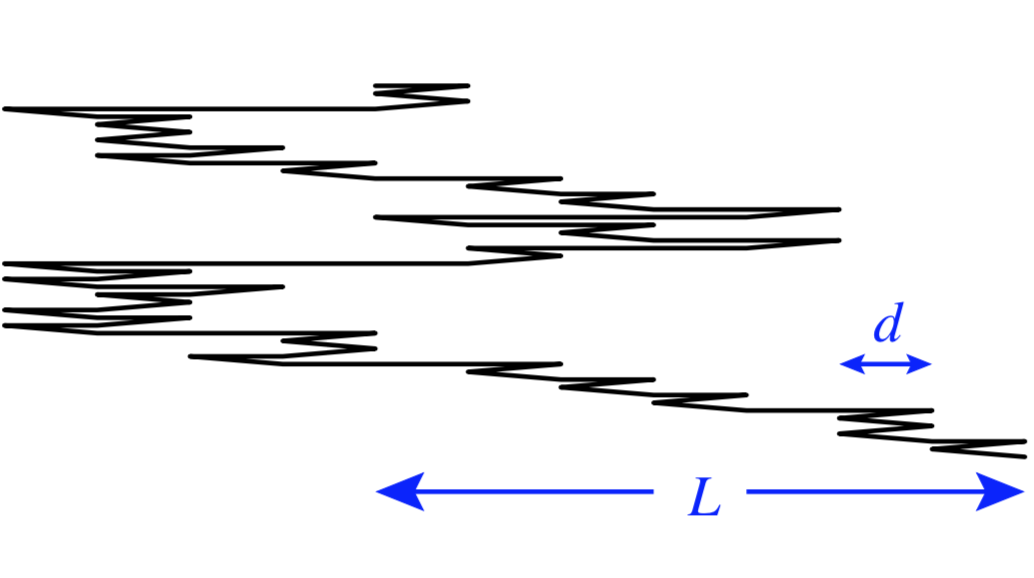
\includegraphics[width=0.5\linewidth]{pset4_fig1}
\caption{Simple model of a rubber band with $N = 100$ segments.\label{fig:1}}
\end{figure}

\begin{question}\textbf{Part (a):}
Find the exact formula for the entropy of this system in terms of $d$, $N$, and $L$.
\end{question}

\begin{solution}
Let $S$ be the entropy. The definition of entropy is given by the Boltzman constant multiplied by the logarithium of accessible microstates $\Omega$ at a given energy $S = k_B\log(\Omega)$. We need a function $\Omega$ such that entropy is maximized when $L=0$, and minimized when $L=Nd$.
Suppose $L=(N-K)d$, where $K$ is the number of ``random'' steps taken to the left. The number of degenerate microstates at this length is given by the binomial coefficient. $\Omega$ is then the sum over all possible values of $N$. We can substitute $K = N - L/d$ to write $\Omega$ in terms of the proper variables, then take the logarithim and we've finished.

\begin{gather}
S = k_B\log \Omega\label{eq:Sdef}
\\
K = N - L/d
\\
\Omega = \binom{N}{K} = \binom{N}{N - L/d} =  \frac{N!}{(\frac{L}{d}!) (N - \frac{L}{d})!}
\\
\boxed{S = k_B \log \Bigg[ \frac{N!}{(\frac{L}{d}!) (N - \frac{L}{d})!}\Bigg]}\label{eq:sol1a}
\end{gather}
\end{solution}

\begin{question}\textbf{Part (b):}
The external world, at temperature $T$, exerts a pulling force on the molecule. The molecule exerts an equal but opposite \emph{entropic} force $F$. (i) Find an expression for the force $F$ exerted by the molecule on the bath in terms of bath entropy. (ii) Using the fact that the length $L$ must maximize the entropy of the Universe, write a general expression for $F$ in terms of the internal entropy $S$ of the molecule.
\end{question}

\begin{solution}
(i) We start with the differential form definition (eq.~\ref{eq:dsde}) to write the bath entropy in terms of energy. The change in energy $dE$ of the rubber molecule is equal to the work done by the pulling force (eq.~\ref{dE}). From here, it is simple to get an expression for force in terms of bath entropy.
\begin{gather}
\pdv{S_\text{bath}}{E} = \frac{1}{T}\label{eq:dsde}
\\
\d{E} = - \vb{F} \cdot \d{\vb{x}} \label{dE}
\\
\d{S_\text{bath}} = - \frac{1}{T} \vb{F} \cdot \d{\vb{x}}
\\
\boxed{F = - T \pdv{S_\text{bath}}{L}}\label{eq:sol1bi}
\end{gather}



\noindent
(ii) At equilibrium, the total entropy $S_\text{bath} + S$ is maximized; the function $S_\text{univ}$ is peaked at the equilibrium value of energy. Thus we can set it's derivative equal to zero.
\begin{align}
S_\text{univ}&= S_\text{bath}(E_1) + S(E - E_1)
\\
\pdv{S_\text{univ}}{E_1}&= \pdv{S_\text{bath}}{E_1} - \pdv{S}{E_2} = 0
\end{align}
For our model, energy is a function of the length displaced; $\d{E} = \vb{F}\cdot\d{\vb{L}}$. Once we make this change of variables, we can substitute eq.~\ref{eq:sol1bi}. Remember that total energy is conserved,\footnote{Hence the minus sign that seems to appear out of nowhere.} $\d{E_1} = - \d{E_2}$.
\begin{align}
\pdv{S_\text{bath}}{E_1} &= \pdv{S}{E_2}
\\
\frac{1}{F}\pdv{S_\text{bath}}{L} &= - \frac{1}{F} \pdv{S}{L}
\end{align}
Satisfying Newton's 3rd axiom,\footnote{For every action, there is an equal but opposite reaction.} we find that the force in terms of the molecule's entropy is \emph{equal, but opposite} to the force in terms of the bath's entropy.
\begin{align}
\Aboxed{F &= T \pdv{S}{L}}\label{eq:sol1bii}
\end{align}

\end{solution}

\newpage
\begin{question}\textbf{Part (c):}
Take eq.~\ref{eq:sol1a}, eq.~\ref{eq:sol1bii} and Stirling's formula to write the force law $F(L)$ for our molecule for large lengths $N$. What is the spring constant $K$ for our molecule for small $L$?
\end{question}

\begin{solution}
The entropic force in terms of internal entropy is $T\pdv*{S}{L}$. For large $L$, we can use Stirling's approximation to simplify eq.~\ref{eq:sol1a}.

\begin{align}
S & = k_B \log \Bigg[ \frac{N!}{(\frac{L}{d}!) (N - \frac{L}{d})!}\Bigg]
\\
& \approx k_B \Bigg[ N\log N - \frac{L}{d}\log\frac{L}{d} - N\log(N - \frac{L}{d}) - \frac{L}{d}\log(N - \frac{L}{d}) \Bigg]
\end{align}
Differentiating with respect to $L$ we get:
\begin{align}
\pdv{S}{L} &= k_B \pdv{L} \Bigg[ N\log N - \frac{L}{d}\log\frac{L}{d} - N\log(N - \frac{L}{d}) - \frac{L}{d}\log(N - \frac{L}{d}) \Bigg]
\\
&= {k_B} \Bigg[ -\frac{1}{d}\log(1 - \frac{L}{dN}) - \frac{1}{d} +  \frac{1 - \frac{dN}{L}}{1 - \frac{dL}{N}} \Bigg] \label{eq:dSdL}
\end{align}
We can rewrite the log term in terms of its Taylor series, $\log(1-x) =-\sum_n x^n/n$. For small lengths $L$, we can take only the first term from the Taylor series. We can also disregard the third term in eq.~\ref{eq:dSdL}; for large $N$, $(1-dN/L)/(1-dL/N)\sim 0$ is a good first order approximation. The second term $-1/d$ is a constant, so we will throw it away for the rest of the discussion.\footnote{Once multiplied by $k_BT$, this term has units of [energy]/[distance] = [force]. It could just be a residual term after making many approximations, or it could be force term caused by the vibrational entropy of the atoms, since it is directly proportional to the temperature $T$ of the rubber.}
\begin{gather}
\log(1-L/dN) = -\sum_n \frac{1}{n}\frac{L^n}{Nd} \approx -\frac{L}{Nd}
\\
\pdv{S}{L} \approx -\frac{k_B}{d} \frac{L}{Nd}
\\
\boxed{
F(L) = T\pdv{S}{L} = -\frac{k_BT}{d^2N} L  \sim -Kx}
\\
\boxed{K = \frac{k_BT}{d^2N}}
\end{gather}
We get a ``spring'' equation $F(L) = -KL$ valid for large $N$ and small $L$
\end{solution}






\begin{question}\textbf{Part (d):}
If we increase the temperature of our rubber band while it is under tension, will it expand or contract? Why?
\end{question}

\begin{solution}
Intuitively, we know that an increase in temperature of the rubber band will increase its entropy. This is a fundamental fact about our Universe. From our model, we know that this increase of internal entropy is associated with a decrease of its length. This is why after we remove an external force from a rubber band, it contracts back to its initial length; entropy never decreases without outside work being put in.
I will attempt to show this mathematically.

Let $\pdv*{L}{T}$ be the change of the molecule's length with respect to its temperature. Using partial gymnastics, we can write this relationship in terms of the molecule's internal entropy $S$.
\begin{align}
\pdv{L}{T} &= \pdv{L}{S} \pdv{S}{T} = \bigg( \pdv{S}{L} \bigg)^{-1} \pdv{S}{T}\label{eq:dLdT}
\end{align}
We can show that $\Delta {S} > 0$ for any change in temperature $\Delta T$.
\begin{gather}
\pdv{S}{T} = \frac{Q}{T}
\\
\Delta S = \int \d{S} = \int_{T_i}^{T_f} \frac{Q}{T} \d{T} = Q\log{\frac{T_f}{T_i}}
\\
\frac{\Delta S}{\Delta T} > 0 \ \text{for positive} \ \Delta T
\end{gather}
Now consider the first term in eq.~\ref{eq:dLdT}. We can tell by looking at eq.~\ref{eq:sol1a} that the molecule's entropy has a maximum when $L = Nd/2$; the function $S(L)$ is sharply peaked at $S(Nd/2)$. Elsewhere, its derivative is negative.
\begin{align}
\pdv{S}{L} \leq 0
\end{align}
Multiplying $(+)$ by $(-)$ always produces $(-)$. We have proved that \boxed{\pdv*{L}{T} < 0.}
\end{solution}


\begin{question}\textbf{Part (e):}
True or false?
\end{question}

\begin{enumerate}

\item \textit{When we stretch the rubber band, it will cool; the configurational entropy of the random walk will decrease, causing the entropy in the vibrations to decrease, causing the temperature to decrease.}
\\
\textbf{False.} The total entropy should stay approximately constant. The configurational entropy decreases but the vibrational entropy should increase, causing the temperature to increase.

\item \textit{When we stretch the rubber band, it will cool; the configurational entropy of the random walk will decrease, causing the entropy in the vibrations to increase, causing the temperature to decrease.}
\\
\textbf{False.} The increase in vibrational entropy should cause the temperature to increase.

\item \textit{When we let the rubber band relax, it will cool; the configurational entropy of the random walk will increase, causing the entropy in the vibrations to decrease, causing the temperature to decrease.}
\\
\textbf{True.}

\item \textit{When we let the rubber band relax, there must be no temperature change, since the entropy is constant.}
\\
\textbf{False.} Although the entropy is constant, there are two forms of entropy in the rubber: configurational and vibrational. The entropy ``flows'' from one to the other when the rubber relaxes. The change in vibrational entropy is responsible for temperature fluctuations.

\item \textit{Like the ideal gas, the temperature changes because of the net work done on the system.}
\\
\textbf{True.}

\item \textit{Unlike the ideal gas, the work done on the rubber band is positive when the rubber band expands.}
\\
\textbf{True.}

\end{enumerate}





%%%%%%%%%%%%%%%%%%%%%%%%%
%% Information Entropy %%
%%%%%%%%%%%%%%%%%%%%%%%%%
\newpage
\section{Information entropy}
Entropy is a measure of your ignorance about a system; it is a measure of the lack of information. Consider the following situation. Your grandparent has sent you an e-mail. From the header, you know it contains 1000 characters. Each character is made of 8 bits, which allows $2^8 = 256$ different letters of symbols per character.

%%%%%%%%%%%%
%% part b %%
%%%%%%%%%%%%

\begin{question}\textbf{Part (a):}
Assuming all possible messages are equally likely, how many different messages $N$ could there be? What is the corresponding upper bound $S_\text{max}$ for the information entropy $k_S\log N$?
\end{question}

\begin{solution}
Each character contains 8 bits. That allows $n = 2^8$ different possible symbols per character. Each symbol is equally likely, thus N is given by $1000 n$.
\begin{align}
N& = 1000n = 1000 \cdot 2^8 = \boxed{256000}
\end{align}
There are 256,000 different messages your grandparent could send you. The corresponding maximum Shannon entropy is found by plugging this maximum $N$ in $S_\text{Shannon} = k_S \log N$.
\begin{align}
\Aboxed{
S_\text{max}& = k_S \log 256000
}
\end{align}
\end{solution}

%%%%%%%%%%%%
%% part b %%
%%%%%%%%%%%%

\begin{question}\textbf{Part (b):}
Your grandparent writes rather dull messages; there are a total of 16 equally likely messages. After you read the message, you forget the details of the wording and only remember these key points of information. (i) What is the actual information entropy change $\Delta S_\text{Shannon}$ you undergo when reading the message? (ii) If your grandparent writes one message per month, what is the minimum number of 8-bit characters per year that it would take to send your grandparent's messages? (You may lump together multiple messages into a single character.)
\end{question}

\begin{solution}
(i) Since we can categorize each letter into one of 16 categories, our new $N$ for the number of possible messages changes. $N_i$ takes on the value of 16. Once we ``observe'' the message, it ``collapses'' into one of the possibilities; $N_f = 1$. Our change in entropy is given by the final entropy minus the initial entropy.
\begin{align}
\Delta S_\text{Shannon}& = S_f - S_i = k_S \big( \log N_f - \log N_i \big)
\\
& = - k_S \log \bigg[ \frac{N_i}{N_f} \bigg]
\\
\Aboxed{
\Delta S_\text{Shannon}& = - k_S \log[16]
}
\end{align}

\bigbreak
\noindent
(ii) To maximize the sad tone of this problem, let's assume the order in which we receive the letters doesn't matter.\footnote{Although footnote 54 in Sethna mentions the letters contain college basketball predictions, this information does not appear to be time sensitive. Since they are making predictions at random without taking into account external factors (e.g. which team has better players this season) I feel like I am justified in making this assumption.}
%~
We have 12 letters to account for, each of which fall into one of 16 categories. There for the number of possible combinations are 16 choose 12.
\begin{gather}
\text{Num combinations} = \binom{16}{12} = 1820
\end{gather}
Let $\mathbb{C} = \{c_1,c_2, \dots, c_{1820}\}$ be the set of all possible combinations. Assign each $c_k$ a particular combination of $N$ bits. We need \emph{at least} $2^N$ bits to represent all of our information.
\begin{align}
2^N& = 1820
\\
\log_2 2^N& = \log_2 1820
\\
N& = \log_2 1820 \simeq 10.82
\end{align}
We need 11 bits to store the information. Each symbol contains 8 bits, so we need two 8-bit symbols needed to store the important information from each letter.
\begin{gather}
	\boxed{
\text{Number of symbols needed} = 2
}
\end{gather}

\end{solution}
























%%%%%%%%%%%%%%%%%%%%%%%%%%%%%%%%%%%%
%% Light emmission and absorption %%
%%%%%%%%%%%%%%%%%%%%%%%%%%%%%%%%%%%%

\section{Light emmision and absorption}


Considering Planck's experiment for deriving the Black Body Radiation equation. (see eq.~\ref{eq:Planck}). Measure the energy radiating out of a small hole, of area $A$. Let us assume the hole is on the upper face of the cavity, perpendicular to $\va{e}_z$.

What is the photon distribution just inside the boundary of the hole? Few photons come into the hole from outside ($v_z < 0$). However, photons with $v_z > 0$ should be unaffected by the presence of the hole.\footnote{Those photons were emitted from far distant walls of the cavity, where the hole is just a negligible pertubation.} Presuming the relevant photons just inside the hole are distributed in the same way as in the box as a whole, how many leave in a time $\d{t}$?

From fig.~\ref{fig:2}, those photons within $v_z\d{t}$ of the boundary will escape in time $\d{t}$. We can relate the photon velocity angle to the verticle by $v_z = c\cos\theta$. The Planck distribution is isotropic, so the probability that a photon will be moving at an angle $\theta$ is the perimeter of the circle $\theta$ on the sphere divided by the area of the sphere.


\begin{figure}[h!]
\centering
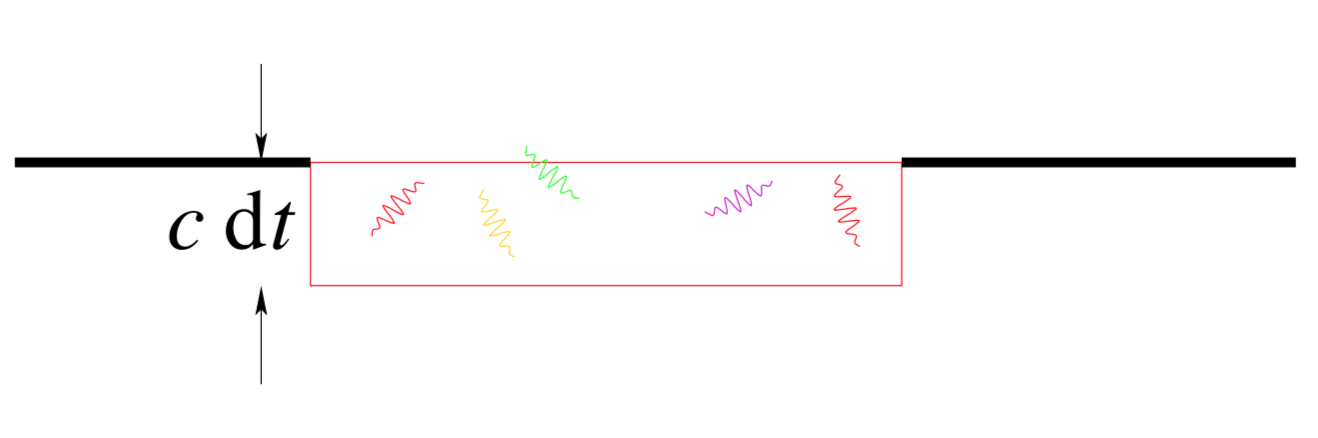
\includegraphics[width=.5\linewidth]{PSet4_Fig2}
\caption{Photon emission from a hole. The photons leaving a cavity in a time $\d{t}$ are those withing $v_z\d{t}$ of the hole.}\label{fig:2}
\end{figure}

\begin{equation}
\begin{aligned}
V u(\omega) \d{\omega}&
= \frac{\hbar \omega g(\omega)}{\exp[\hbar\omega/k_BT] - 1} \d{\omega}
\\
&
= \frac{V\hbar}{\pi^2c^3}\frac{\omega^3 \d{\omega}}{\exp[\hbar\omega/k_BT] - 1}
\label{eq:Planck}
\end{aligned}
\end{equation}
\begin{center}
\text{{\small \textbf{Equation 3.1:} Planck's formula for black-body radiation.}}
\end{center}



\newpage

\begin{question}\textbf{Part (a):}
Show that the probability density $\rho(v_z)$ for a particular photon to have velocity $v_z$ is independent of $v_z$ in the range $(-c,c)$, and this is $1/2c$.
\end{question}

\begin{solution}
Let $\rho(v_z)$ be the probability distribution of a photon having a velocity of $v_z$. $p(v_z)$ is normalized, such that $\int \rho(v_z) \d{v_z} = 1$. All $v_z$ are equally probable because the Planck distribution is isotropic. In our normalization integral, we can make a change of variables from $v_z$ to $\theta$, and we will find that $\rho(v_z)$ must be independent of $v_z$ for the range $(-c,c)$.
\begin{align}
1 &= \int_{-c}^c \rho(v_z) \d{v_z}
\end{align}
Let $v_z = c \cos\theta$, $\d{v_z} = -c \sin\theta\d{\theta}$.
\begin{align}
1 &= -c \int_{-\pi}^{0} \rho(\theta) \sin\theta \d{\theta} = c \int_{0}^{-\pi} \rho(\theta) \sin\theta \d{\theta}
\end{align}
If $\rho$ is independent of $v_z$ and $\theta$, then
\begin{align}
1 &= c \rho \int_{0}^{-\pi} \sin\theta \d{\theta} = c \rho \cos{\theta} \eval_{-\pi}^{0} = 2c\rho
\end{align}
Therefore, $\boxed{\rho(v_z) = \frac{1}{2c}}$.
\end{solution}



\begin{question}\textbf{Part (b):}
An upper bound on the energy emitted from a hole of area $A$ is given by the energy in the box as a whole (eq.~\ref{eq:Planck}) times the fraction $Ac\d{t}/V$ of the volume within $c\d{t}$ of the hole. Show that the actual energy emitted is 1/4 of this upper bound.
\end{question}


\begin{solution}
The upper bound of energy emitted occurs if all of the photons within $c\d{t}$ of the hole are traveling at $v_z = c$.
\begin{equation}
E_\text{upper} = \frac{V\hbar}{\pi^2c^3}\frac{\omega^3 \d{\omega}}{\exp[\hbar\omega/k_BT] - 1} \frac{Ac\d{t}}{V}
\end{equation}
However, we stated previously that all possible $v_z$ are equally probable. The real energy emmitted is given by multipling eq.~\ref{eq:Planck} by the volume ratio $Al/V$. $l$ is the average distance traveled by photons, equal to $\d{t}\int v_z \rho(v_z) \d{v_z}$
\begin{align}
\begin{aligned}
E &= \frac{V\hbar}{\pi^2c^3}\frac{\omega^3 \d{\omega}}{\exp[\hbar\omega/k_BT] - 1} \frac{A\d{t}}{V} \int_{0}^{c} v_z \rho(v_z) \d{v_z}
\\
&= \frac{V\hbar}{\pi^2c^3}\frac{\omega^3 \d{\omega}}{\exp[\hbar\omega/k_BT] - 1} \frac{A\d{t}}{2cV} \int_{0}^{c} v_z \d{v_z}
\\
&= \frac{V\hbar}{\pi^2c^3}\frac{\omega^3 \d{\omega}}{\exp[\hbar\omega/k_BT] - 1} \frac{cA\d{t}}{4V}
\\
\Aboxed{
E &= 1/4 E_\text{upper}}
\end{aligned}
\end{align}

Hence the power per unit area emmitted from the small hole in equilibrium is
\begin{gather}
P_\text{black}(\omega,T) = \frac{c}{4} \frac{\hbar}{\pi^2c^3}\frac{\omega^3\d{\omega}}{\exp[\hbar\omega/k_BT] - 1}\label{eq:power}.
\end{gather}
\end{solution}


\newpage
\begin{question}\textbf{Part (c):}
Using the fact $\int_0^\infty x^3/(\text{e}^x - 1)\d{x} = \pi^4/15$, show that
$
Q_\text{tot}(T) = \int_0^\infty P_\text{black}(\omega,T)\d{\omega} = \sigma T^4
$
and give a formula for the Stefan-Boltzmann constant $\sigma$.
\end{question}

\begin{solution}
The total power per unit area at temperature $T$ is given by integrating eq.~\ref{eq:power} over all frequencies.

\begin{align}
Q_\text{tot}(T) &= \int_0^\infty P_\text{black}(\omega,T)\d{\omega}
\end{align}
Let $ \hbar \omega/k_BT = x$, $\hbar\d{\omega}/k_BT = \d{x}$.
\begin{gather}
	\begin{aligned}
Q_\text{tot} &= \frac{c}{4} \frac{\hbar}{\pi^2c^3} \bigg( \frac{k_BT}{\hbar} \bigg)^4 \int_0^\infty \frac{1}{\text{e}^x - 1} \d{x}
\\
&= \frac{c}{4} \frac{\hbar}{\pi^2c^3} \bigg( \frac{k_BT}{\hbar} \bigg)^4 \bigg( \frac{\pi^4}{15} \bigg)
\\
&= \frac{\pi^2}{60}\bigg( \frac{k_B^4}{c^2 \hbar^3}\bigg) \cdot T^4
\end{aligned}
\\
\boxed{Q_\text{tot} = \sigma T^4}
\\
\boxed{\sigma = \frac{\pi^2}{60}\bigg( \frac{k_B^4}{c^2 \hbar^3}\bigg)}
\end{gather}

\end{solution}

\end{document}
